\documentclass[tikz,convert={outfile=\jobname.svg}]{standalone}
\begin{document}
   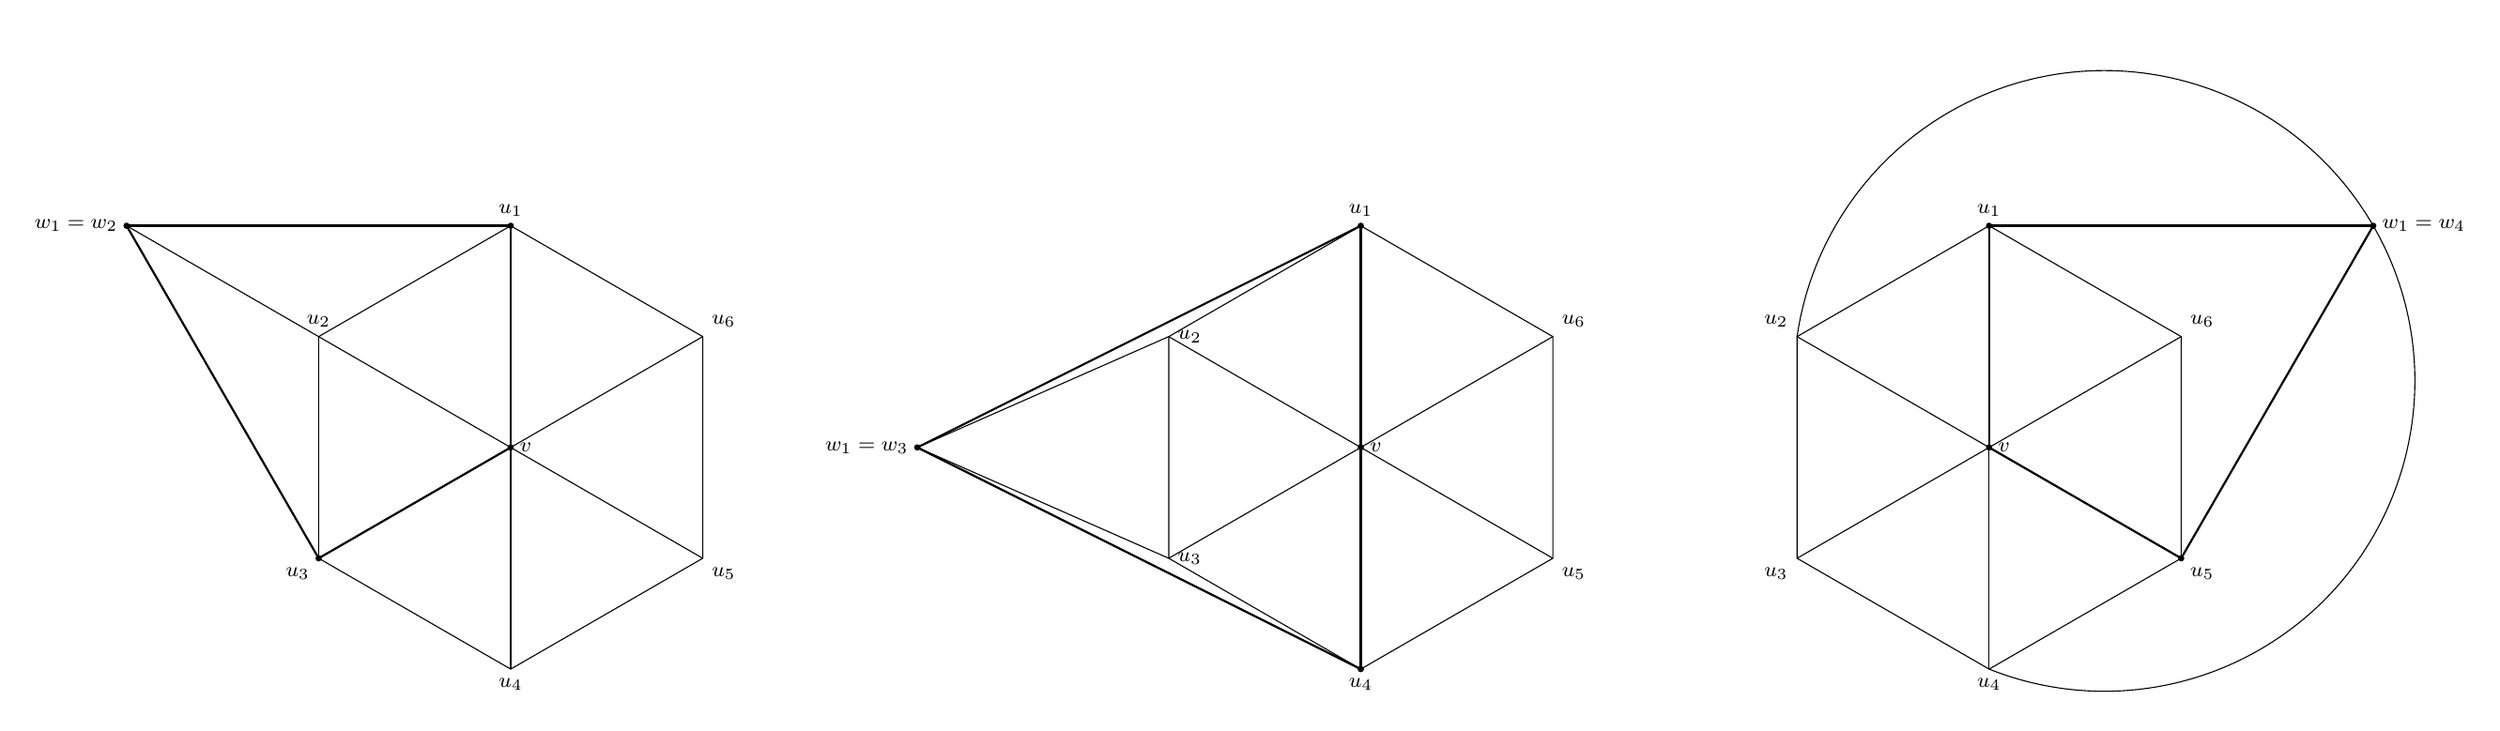
\begin{tikzpicture}
      \def\R{3cm}
      \begin{scope}
         \draw (0, 0) node[anchor=west]{\footnotesize$v$};
         \draw (90: \R) node[anchor=south]{\footnotesize$u_1$};
         \draw (150: \R) node[anchor=south]{\footnotesize$u_2$};
         \draw (210: \R) node[anchor=north east]{\footnotesize$u_3$};
         \draw (270: \R) node[anchor=north]{\footnotesize$u_4$};
         \draw (330: \R) node[anchor=north west]{\footnotesize$u_5$};
         \draw (30: \R) node[anchor=south west]{\footnotesize$u_6$};
         \foreach \x in {30, 90, ..., 330} {
            \draw (0, 0) -- (\x: \R);
         }
         \draw (30: \R) \foreach \x in {90, 150, ..., 330} {
            -- (\x: \R)
         } -- cycle;
         \filldraw[black] (0, 0) circle(1pt);
         \filldraw[black] (90: \R) circle(1pt);
         \filldraw[black] (150: 2*\R) circle(1pt) node[anchor=east]{\footnotesize$w_1 = w_2$};
         \filldraw[black] (210: \R) circle(1pt);
         \draw[thick] (0, 0) -- (90: \R);
         \draw[thick] (90: \R) -- (150: 2*\R);
         \draw[thick] (150: 2*\R) -- (210: \R);
         \draw[thick] (210: \R) -- (0, 0);
         \draw (150: 2*\R) -- (150: \R);
      \end{scope}
      \begin{scope}[xshift=11.5cm]
         \draw (0, 0) node[anchor=west]{\footnotesize$v$};
         \draw (90: \R) node[anchor=south]{\footnotesize$u_1$};
         \draw (150: \R) node[anchor=west]{\footnotesize$u_2$};
         \draw (210: \R) node[anchor=west]{\footnotesize$u_3$};
         \draw (270: \R) node[anchor=north]{\footnotesize$u_4$};
         \draw (330: \R) node[anchor=north west]{\footnotesize$u_5$};
         \draw (30: \R) node[anchor=south west]{\footnotesize$u_6$};
         \foreach \x in {30, 90, ..., 330} {
            \draw (0, 0) -- (\x: \R);
         }
         \draw (30: \R) \foreach \x in {90, 150, ..., 330} {
            -- (\x: \R)
         } -- cycle;
         \filldraw[black] (0, 0) circle(1pt);
         \filldraw[black] (90: \R) circle(1pt);
         \filldraw[black] (180: 2*\R) circle(1pt) node[anchor=east]{\footnotesize$w_1 = w_3$};
         \filldraw[black] (270: \R) circle(1pt);
         \draw[thick] (0, 0) -- (90: \R);
         \draw[thick] (90: \R) -- (180: 2*\R);
         \draw[thick] (180: 2*\R) -- (270: \R);
         \draw[thick] (270: \R) -- (0, 0);
         \draw (180: 2*\R) -- (150: \R);
         \draw (180: 2*\R) -- (210: \R);
      \end{scope}
      \begin{scope}[xshift=20cm]
         \draw (0, 0) node[anchor=west]{\footnotesize$v$};
         \draw (90: \R) node[anchor=south]{\footnotesize$u_1$};
         \draw (150: \R) node[anchor=south east]{\footnotesize$u_2$};
         \draw (210: \R) node[anchor=north east]{\footnotesize$u_3$};
         \draw (270: \R) node[anchor=north]{\footnotesize$u_4$};
         \draw (330: \R) node[anchor=north west]{\footnotesize$u_5$};
         \draw (30: \R) node[anchor=south west]{\footnotesize$u_6$};
         \foreach \x in {30, 90, ..., 330} {
            \draw (0, 0) -- (\x: \R);
         }
         \draw (30: \R) \foreach \x in {90, 150, ..., 330} {
            -- (\x: \R)
         } -- cycle;
         \filldraw[black] (0, 0) circle(1pt);
         \filldraw[black] (90: \R) circle(1pt);
         \filldraw[black] (30: 2*\R) circle(1pt) node[anchor=west]{\footnotesize$w_1 = w_4$};
         \filldraw[black] (330: \R) circle(1pt);
         \draw[thick] (0, 0) -- (90: \R);
         \draw[thick] (90: \R) -- (30: 2*\R);
         \draw[thick] (30: 2*\R) -- (330: \R);
         \draw[thick] (330: \R) -- (0, 0);
         \draw (30: 2*\R) arc(30: 171.8: 4.2001);
         \draw (30: 2*\R) arc(30: -111.8: 4.2001);
      \end{scope}
   \end{tikzpicture}
\end{document}
